\documentclass[a4paper,12pt]{scrartcl}
\usepackage{framed}
\usepackage{enumitem}
\usepackage{todonotes}

\usepackage[utf8]{inputenc}
\usepackage{amsfonts}
\usepackage{listings}
\usepackage{hyperref}
\usepackage{listings}
\usepackage{color}
\definecolor{verylightgray}{RGB}{244,244,244}
\definecolor{lightgray}{RGB}{232,232,232}
\definecolor{listinggray}{gray}{0.9}
\definecolor{lbcolor}{rgb}{0.9,0.9,0.9}
\definecolor{gray}{rgb}{0.4,0.4,0.4}
\definecolor{darkblue}{rgb}{0.0,0.0,0.6}
\definecolor{cyan}{rgb}{0.0,0.6,0.6}
\definecolor{dkblue}{rgb}{0,0.1,0.5}
\definecolor{dkgreen}{rgb}{0,0.4,0}
\newcommand{\code}[1]{\colorbox{listinggray}{\texttt{#1}}}
\lstset
{
  captionpos=b,
  basicstyle=\small\ttfamily,
  columns=fullflexible,
  showstringspaces=false,
  commentstyle=\color{gray}\upshape,
  numbers=left,
  stepnumber=1,
  tabsize=2,
  keepspaces=true,
  frame=lines,
  keywordstyle=\color{blue},
  framesep=2pt,
  prebreak=\raisebox{0ex}[0ex][0ex]{\ensuremath{\hookleftarrow}},
  breakindent=4em,
  breaklines=true
}
\lstdefinelanguage{CPP}
{
 morecomment = [l][\color{dkgreen}]{//}, 
 morecomment = [l][\color{dkgreen}]{///},
 morecomment = [s][\color{dkgreen}]{/*}{*/},
 morestring=[b]", 
 sensitive = true,
 morekeywords = {abstract,  event,  new,  struct,
   as,  explicit,  null,  switch,
   base,  extern,  object,  this,
   bool,  false,  operator,  throw,
   break,  finally,  out,  true,
   byte,  fixed,  override,  try,
   case,  float,  params,  typeof,
   catch,  for,  private,  uint,
   char,  foreach,  protected,  ulong,
   checked,  goto,  public,  unchecked,
   class,  if,  readonly,  unsafe,
   const,  implicit,  ref,  ushort,
   continue,  in,  return,  using,
   decimal,  int,  sbyte,  virtual,
   default,  interface,  sealed,  volatile,
   delegate,  internal,  short,  void,
   do,  is,  sizeof,  while,
   double,  lock,  stackalloc,   
   else,  long,  static,   
   enum,  namespace,  string, template, typename, include, nullptr, chan, clock},
 emph={},
 emphstyle=\color{blue},
 emph={[2]value},
 emphstyle={[2]\textbf}
}

\title{Verification mini-project}
\subtitle{Crossing the River}
\author{Jacob Karstensen Wortmann\\Sam Sepstrup Olesen\\Nicklas Andersen\\\textit{sw805f14}}

\begin{document}
\maketitle %project description

\section*{Introduction}
The purpose of the exercise is to model a game, Crossing the River, in UPPAAL. The goal of the game is to get a group of people from one riverside to the other. The group consists of two daughters, two sons, a mom, a dad, a Police Officer, and a thief.
The game has a list of rules that must be followed at all times to complete the game:

\begin{itemize}
\item Max 2 persons on the boat,
\item Mom not alone with boys,
\item Dad not alone with girls,
\item Thief not alone with family,
\item Only the Police Officer, dad and mom can handle the boat.
\end{itemize}

The following is the specification for our system. It simply checks whether a trace exists where all people are on the right side of the river.
\begin{lstlisting}[keywords={and, E}]
E<> (Police.right and Thief.right and Dad.right and Mom.right
and Boy1.right and Boy2.right and Girl1.right and Girl2.right)
\end{lstlisting}

\section*{Boat}
\begin{figure}[h!]
\centering
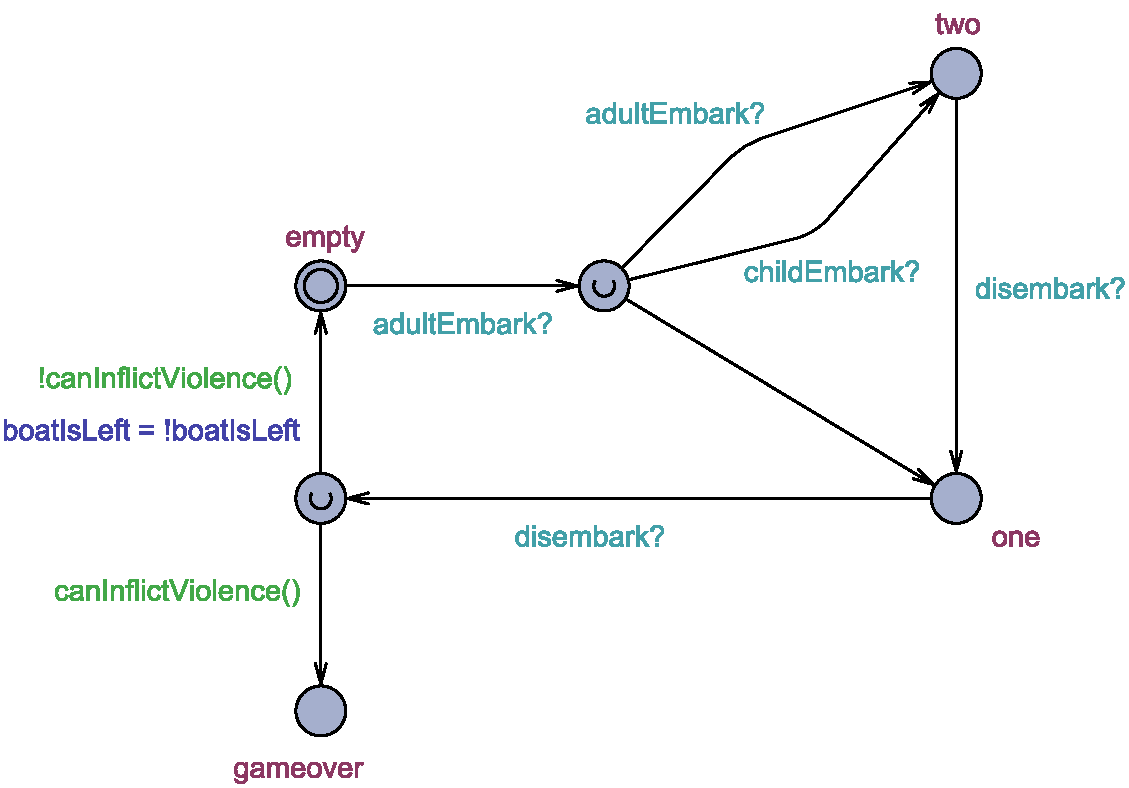
\includegraphics[width=\linewidth]{Boat.pdf}
\caption{Boat automata.}
\label{fig:boat}
\end{figure}

Figure \ref{fig:boat} shows the automata of the boat. The rules of the game defines that an adult needs to be on the boat for it to sail. To conform to this rule our automata require an adult to embark to boat before a second person is allowed to embark. When people on the boat disembark, we check whether this new state conforms to the rules. If it is an allowed state we update the location of the boat. If it is not a valid state the automata goes to a \code{gameover} location, which will cause a deadlock.


\section*{Global declarations}

\begin{lstlisting}[language=CPP, label = lst:plugin_example, caption = Global declaration.]
clock time;

chan adultEmbark, childEmbark, disembark;

bool boatIsLeft = true;

bool policeIsLeft = true;
bool thiefIsLeft  = true;
bool dadIsLeft    = true;
bool momIsLeft    = true;
bool boy1IsLeft   = true;
bool boy2IsLeft   = true;
bool girl1IsLeft  = true;
bool girl2IsLeft  = true;


bool canInflictViolence() {
    if (((momIsLeft == boy1IsLeft) || (momIsLeft == boy2IsLeft))
    	&& (momIsLeft != dadIsLeft))
        return true;

    if (((dadIsLeft == girl1IsLeft) || (dadIsLeft == girl2IsLeft))
    	&& (dadIsLeft != momIsLeft))
        return true;

    if (((thiefIsLeft == boy1IsLeft) || (thiefIsLeft == boy2IsLeft)
    	|| (thiefIsLeft == girl1IsLeft) || (thiefIsLeft == girl2IsLeft)
    	|| (thiefIsLeft == dadIsLeft) || (thiefIsLeft == momIsLeft))
    	&& (thiefIsLeft != policeIsLeft))
        return true;

    return false;
}
\end{lstlisting}

In the the global declarations we define a clock \code{time} which can be used to see how fast a given trace is. \code{time} is not used by the system.

The global declaration also declares the channels and defines the location of the boat and all the people. \code{canInflictViolence} is a function that can be used to check whether the current state is invalid. 

\section*{Police \& Thief}

\begin{figure}[h!]
\centering
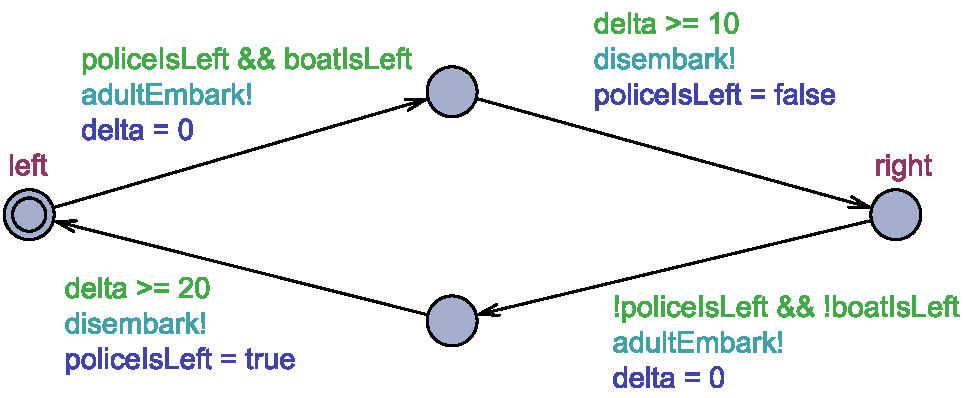
\includegraphics[width=0.7\linewidth]{Police.pdf}
\caption{Police automata.}
\label{fig:police}
\end{figure}

As seen in Figure \ref{fig:police} the Police Officer can move from the left location to the right location. The first transition has a guard that checks that both the Police Officer and the Boat is at the left location. If the guard is true we can proceed by telling the Boat that an adult has embarked and set the \code{delta} (time) value to 0. When the Police Officer disembarks on the other side we specify that it must have taken longer than 10 time units and that the Police Officer is no longer on the left side.
We do the same thing from right to left, except that we specify it must take more than 20 time units to go from right to left, this is to simulate headwind on the river.

\begin{figure}[h!]
\centering
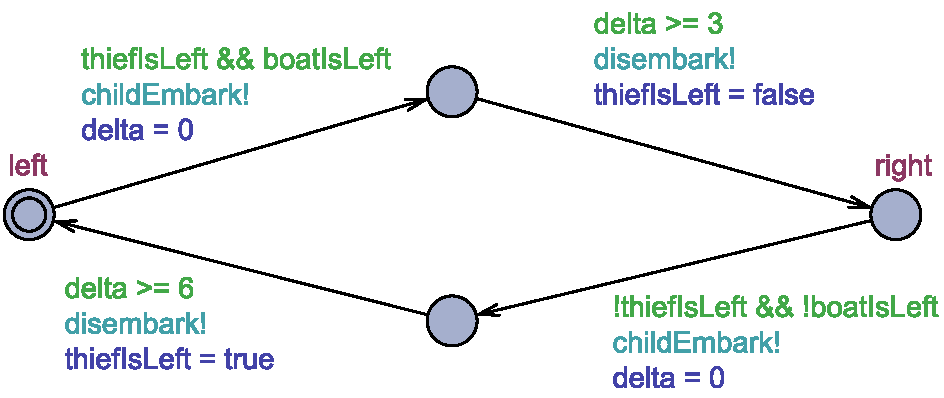
\includegraphics[width=0.7\linewidth]{Thief.pdf}
\caption{Thief automata.}
\label{fig:thief}
\end{figure}

As seen in Figure \ref{fig:thief} the Thief is very similar to the Police Officer, the only differences is that a Thief is treated as a child instead of an adult and that a Thief travels much faster. The reason why the Thief is treated as a child is that the rules of the game specifies that the Thief can not operate the boat.

\section*{Parents \& children}

\begin{figure}[h!]
\centering
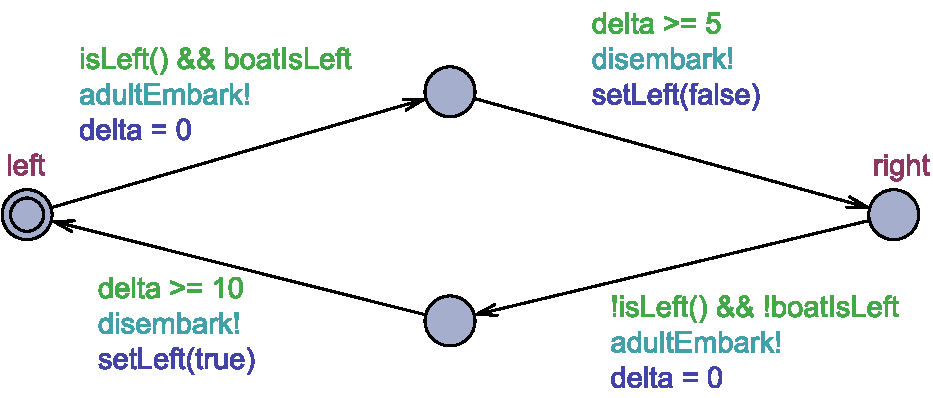
\includegraphics[width=0.7\linewidth]{Parent.pdf}
\caption{Parent automata.}
\label{fig:parent}
\end{figure}

As seen in Figure \ref{fig:parent} the only difference from the \code{Police} is that we call the function \code{isLeft()} to check whether he/she is on the left side or not, the time it takes to sail from side to side is also different. The reason for the \code{isLeft()} function is that we need to know whether the \code{Parent} represents the mother or the father.

\code{Children} works just like the parents except that they are treated as children instead of adults. 
To initialise the \code{Children} it requires two arguments, one to specify whether it is a girl or a boy and the other to specify whether it is the first or second child. When \code{isLeft()} is called it checks the local variables and returns the result for the child.

\begin{lstlisting}[language=CPP, label = lst:plugin_example, caption = Parent declaration.]
clock delta;

bool isLeft() {
    if (isDad)
        return dadIsLeft;
    else
        return momIsLeft;
}

void setLeft(bool left) {
    if (isDad)
        dadIsLeft = left;
    else
        momIsLeft = left;
}
\end{lstlisting}

\begin{figure}[h!]
\centering
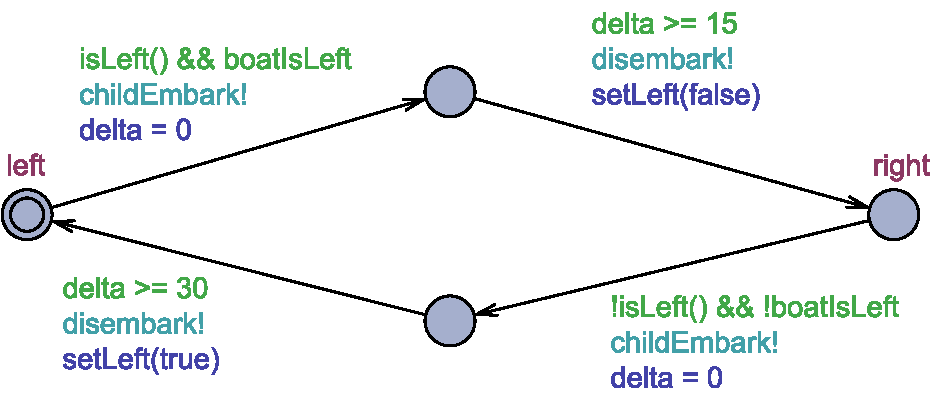
\includegraphics[width=0.7\linewidth]{Child.pdf}
\caption{Child automata.}
\label{fig:child}
\end{figure}

\begin{lstlisting}[language=CPP, label = lst:plugin_example, caption = Child declaration.]
clock delta;

bool isLeft() {
    if (isBoy)
        if (isFirst)
            return boy1IsLeft;
        else
            return boy2IsLeft;
    else
        if (isFirst)
            return girl1IsLeft;
        else
            return girl2IsLeft;
}

void setLeft(bool left) {
    if (isBoy)
        if (isFirst)
            boy1IsLeft = left;
        else
            boy2IsLeft = left;
    else
        if (isFirst)
            girl1IsLeft = left;
        else
            girl2IsLeft = left;
}
\end{lstlisting}


\section*{Additional children}
It is obvious that the system wont allow for multiple thieves since the Police Officer can only able to be on one side at a time and the boat can only transport one thief at a time, making it impossible to send a thief to the other side.

When adding a boy (or a girl), UPPAAL is unable to find a trace that conforms to the rules. You can argue that if it is impossible to move 3 boys to the other side, it is also impossible to move more than 3 boys, since those problems also require that 3 boys are moved to the other side which is proved impossible.

\begin{lstlisting}[language=CPP, label = lst:plugin_example, caption = Global declarations with an extra boy.]
clock time;

chan adultEmbark, childEmbark, disembark;

bool boatIsLeft = true;

bool policeIsLeft = true;
bool thiefIsLeft  = true;
bool dadIsLeft    = true;
bool momIsLeft    = true;
bool boy1IsLeft   = true;
bool boy2IsLeft   = true;
bool boy3IsLeft   = true;
bool girl1IsLeft  = true;
bool girl2IsLeft  = true;


bool canInflictViolence() {
    if (((momIsLeft == boy1IsLeft) || (momIsLeft == boy2IsLeft)
    	|| (momIsLeft == boy3IsLeft))
    	&& (momIsLeft != dadIsLeft))
        return true;

    if (((dadIsLeft == girl1IsLeft) || (dadIsLeft == girl2IsLeft))
    	&& (dadIsLeft != momIsLeft))
        return true;

    if (((thiefIsLeft == boy1IsLeft) || (thiefIsLeft == boy2IsLeft)
    || (thiefIsLeft == boy3IsLeft)
    || (thiefIsLeft == girl1IsLeft) || (thiefIsLeft == girl2IsLeft)
    || (thiefIsLeft == dadIsLeft) || (thiefIsLeft == momIsLeft))
    && (thiefIsLeft != policeIsLeft))
        return true;

    return false;
}
\end{lstlisting}


\end{document}